\chapter[OpenSCAD]{\texttt{OpenSCAD}}

\lettrine[ante=\raisebox{-2ex}{\Large ---},lines=2]{E}{n un principio}
lo intenté con
\texttt{FreeCAD}\footnote{\url{https://www.freecadweb.org/}}
---confesó An\-to\-\mbox{nia---.} Pero no tardé mucho en comprender
que no era la herramienta adecuada.

---¿Probaste entonces con el \texttt{Fusion3D}, o con el
\texttt{Solid\-Works}? ---pre\-gun\-tó ingenuamente Cecilia, y al ver la
cara de Antonia se arrepintió inmediatamente.

---¿¿Qué??  ¿¿¿Programas propietarios???  ---replicó su amiga,
indignada. Cecilia pudo ver que iba a seguir en el mismo tono, pero
con sorpresa apreció que se contuvo. Antonia cerró los ojos y,
haciendo un esfuerzo, suspiró---. En fin, disculpame
---susurró---. Supongo que también son buenos programas, pero ya sabés
que no me siento cómoda más que con programas de código fuente
abierto. Sí, es un capricho, lo sé ---admitió---; pero, ¿qué
querés...? ---y Antonia completó la idea encogiéndose de hombros.

Cecilia, con una sonrisa, la invitó a continuar.

---Entonces fue que encontré
\texttt{OpenSCAD}\footnote{\url{https://www.openscad.org/}} ---el tono
de Antonia recobró su ímpetu natural---. No sabés; está buenísimo. No
creás objetos 3D con el ratón, ni con botones de un menú: los creás
programando, escribiendo. Todo lo creás con texto; el ratón apenas lo
usás para rotar o desplazar la escena que vas creando.

Se notaba en el tono vibrante de la voz de Antonia que estaba
conmovida. A Cecilia le costaba imaginar porqué alguien podía verse
motivado por lo que en última instancia no era otra cosa que una
limitación, tal como es la imposibilidad de usar el ratón, los botones
y los menúes. Pero hasta en la locura de Antonia había una lógica; tal
vez retorcida, tal vez excéntrica, pero una lógica al fin. Y, por otra
parte, el mágico objeto que guiaba la luz del Sol seguía ahí, en sus
manos: dócil, mudo y todavía secreto. Así que la dejó continuar.

\begin{figure}[ht]
  \centering  
  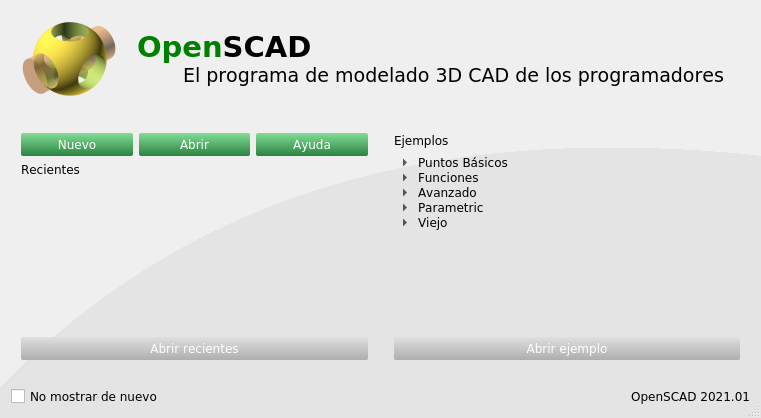
\includegraphics[width=.85\textwidth]{imagenes/openscad-bienvenida}  
  \caption{Pantalla de bienvenida de \openscad.}
\end{figure}

---Cuando abrís \openscad{} aparece una ventana no muy distinta a la
de tantos otros programas ---adelantó An\-to\-\mbox{nia---.} En ella se te ofrece
la opción de comenzar con un texto nuevo, abrir uno ya escrito por vos
u otra persona, o incluso chusmear entre una gran cantidad de
ejemplos.


\begin{figure}[t]
  \centering  
  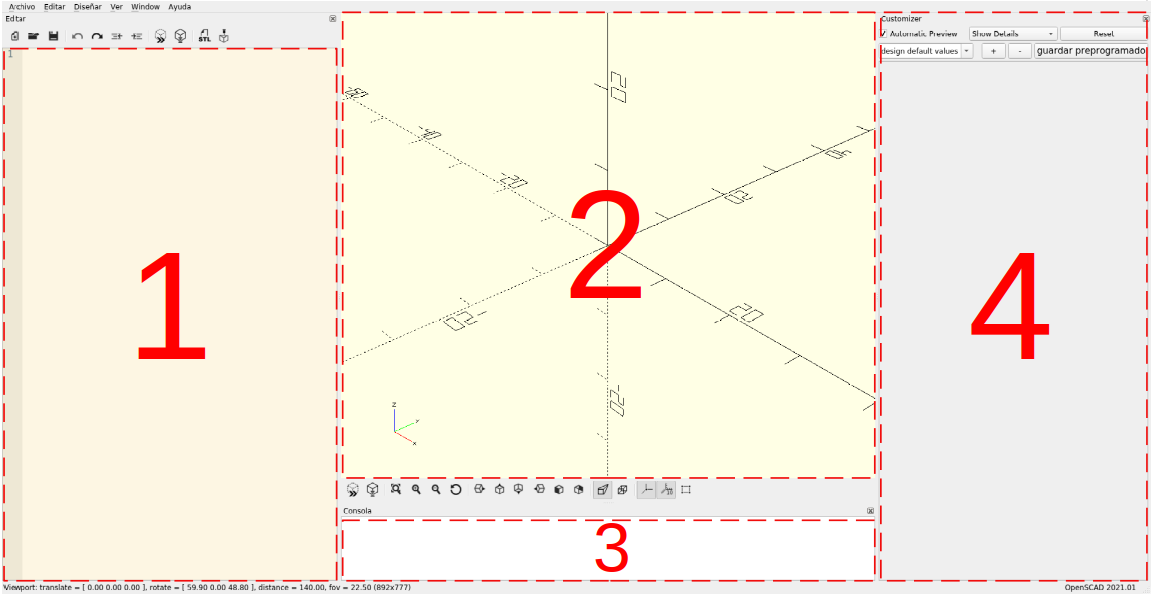
\includegraphics[width=1\textwidth]{imagenes/openscad-pantalla-anotada}
  \caption{Área de trabajo de \openscad.}
  \label{fig:area-trabajo-openscad}
\end{figure}


\guillemotright Si elegís empezar un texto nuevo aparecerá una ventana
dividida en otras cuatro ---agregó Antonia, señalando el monitor de la
computadora con el mentón, que lucía como en la figura
\ref{fig:area-trabajo-openscad}---. En la izquierda (\emph{1})
escribís tu texto, en la central (\emph{2}) se ve el resultado del
mismo y en la de abajo (\emph{3}) aparecen mensajes ocasionales, que
pueden sancionar errores o confirmar el éxito. Te aconsejo que cierres
la de la derecha (\emph{4}) pulsando sobre la pequeña `\texttt{x}' de
su esquina superior derecha: su uso puede serte de utilidad, pero sólo
más adelante.

Cecilia no pudo evitar sentir una suerte de delicioso vértigo ante la
página en blanco que el monitor lanzaba a su rostro.

---¿Qué onda los ejemplos que trae \openscad{}? ---preguntó.

---Están buenísimos. Pero espero que no los entiendas para nada
---contestó Antonia, con un gesto malicioso.

---¡Hey! ¿Por qué? ---preguntó Cecilia, visiblemente asombrada.

---Porque si los entendés por tu cuenta, ¿a quién le voy a contar cómo
hice el reloj solar? ---remató Antonia sonriendo con los ojos y
haciendo, una vez más, pucherito.


%%% Local Variables:
%%% mode: latex
%%% TeX-master: "../libro"
%%% End:
